\chapter{Laws and Metrics}
\label{ch:laws_and_metrics}

Starting off with some terminology, we will introduce some basic concepts and metrics that are fundamental to understanding the performance of parallel systems. We will then delve into the laws that govern the performance of parallel systems, and how they can be used to predict the performance of a parallel system.

\section{Terminology}

\begin{paracol}{2}
   \begin{definition}
      [Speedup]
      The speedup ($S$) is defined as the quotient of the time taken using a single processor ($T (1)$) over the time measured using $p$ processors ($T (p)$)
      \begin{equation}
         S = \frac{T(1)}{T(p)}
      \end{equation}
   \end{definition}
   
   The best speedup we can achieve is $p$, which is the number of processors. This is known as \textbf{linear speedup}.
   Exceptions to this are to as \textbf{superlinear speedup}.
   \switchcolumn

   \begin{figure}[htbp]
      \centering
      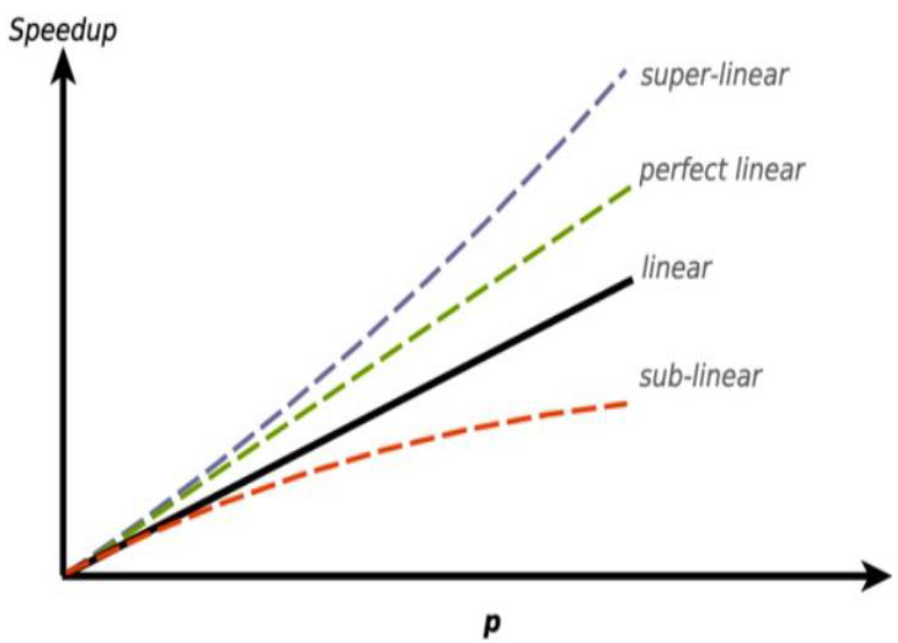
\includegraphics{images/06/speedup.png}
      \caption{Speedup categories}
      \label{fig:06/speedup}
   \end{figure}

\end{paracol}

\begin{definition}
   [Efficiency]
   The efficiency ($E$) is defined as the speedup divided by the number of processors
   \begin{equation}
      E = \frac{S}{p} = \frac{T(1)}{p \cdot T(p)}
   \end{equation}
\end{definition}

$p \cdot T(p)$ is also called \textit{``cost of parallelization''}, or simply \textit{``cost''}. Clearly, the ideal efficiency is 1.

Scalability and speedup are apparently defined in the same way, but there is a significant difference.

\begin{definition}
   [Scalability]
   Scalability considers as $T(1)$ the time obtained by executing the \textbf{parallel} implementation of the algorithm on a single processor.\\
   It is also called \textbf{``relative speedup''}
   \begin{equation}
      Scalability = \frac{T_{par}(1)}{T_{par}(p)}
   \end{equation}
\end{definition}

\begin{definition}
   [Absolute Speedup]
   (Absolute) Speedup instead considers $T(1)$ as the time obtained by executing the ---best--- \textbf{sequential} implementation of the algorithm on a single processor.
   \begin{equation}
      Speedup = \frac{T_{seq}(1)}{T_{par}(p)}
   \end{equation}
\end{definition}

\subsection{Strong and Weak Scaling}
\begin{itemize}
   \item \textbf{Strong-scaling} - the problem size is fixed. Linear scaling is hard to achieve due to \textit{Amdahl's Law}. (discussed later on).
   It depends on the amount of \textbf{serial work}, i.e. the part of the problem that cannot be parallelized.
   \item \textbf{Weak-scaling} - the problem size is $p$ times bigger in the same amount of time. The problem size remains constant per processor, but Weak scaling assumes that as the size of the problem increases, 
   \begin{itemize}
      \item the amount of serial work remains constant (or increases slowly)
      \item The amount of communication among processors remains constant (or increases slowly)
   \end{itemize}
\end{itemize}

Consider the following example:
\begin{itemize}
   \item \texttt{INPUT} - Array $A$ of $n$ numbers
   \item \texttt{OUTPUT} - $\sum_{i=0}^{n-1}$
   \item \texttt{Task} - Parallelize this problem by using an array of \textit{processing elements (PEs)}.
\end{itemize}

\labelitemize{Assumptions}{
   \begin{itemize}
      \item \textbf{Computation}: Each PE can add two numbers stored in its local memory in 1 sec
      \item \textbf{Communication}: A PE can send data from its local memory to the local memory of any other PE in 3 sec (independently of the data size!)
      \item \textbf{Input and Output}: At the beginning of the program, the whole input array A is stored in PE \#0. At the end, the result must be gathered in PE \#0
      \item \textbf{Synchronization}: All PEs operate in a lock-step manner; i.e., they can either compute, communicate, or be idle (no computation-to-communication overlap!).
   \end{itemize}
}

First of all we must establish the sequential runtime ($p=1$), for example $T(1,n) = n-1 sec$.
Then we may evaluate speedup, efficiency, and scalability for different values of $p$.

In the data displayed in the slides, speedup and efficiency decreases for values of $p$ greater than 2. In fact, in the following figure \ref{fig:06/scalability_analysis} we have a figure summarizing results.

\begin{figure}[htbp]
   \centering
   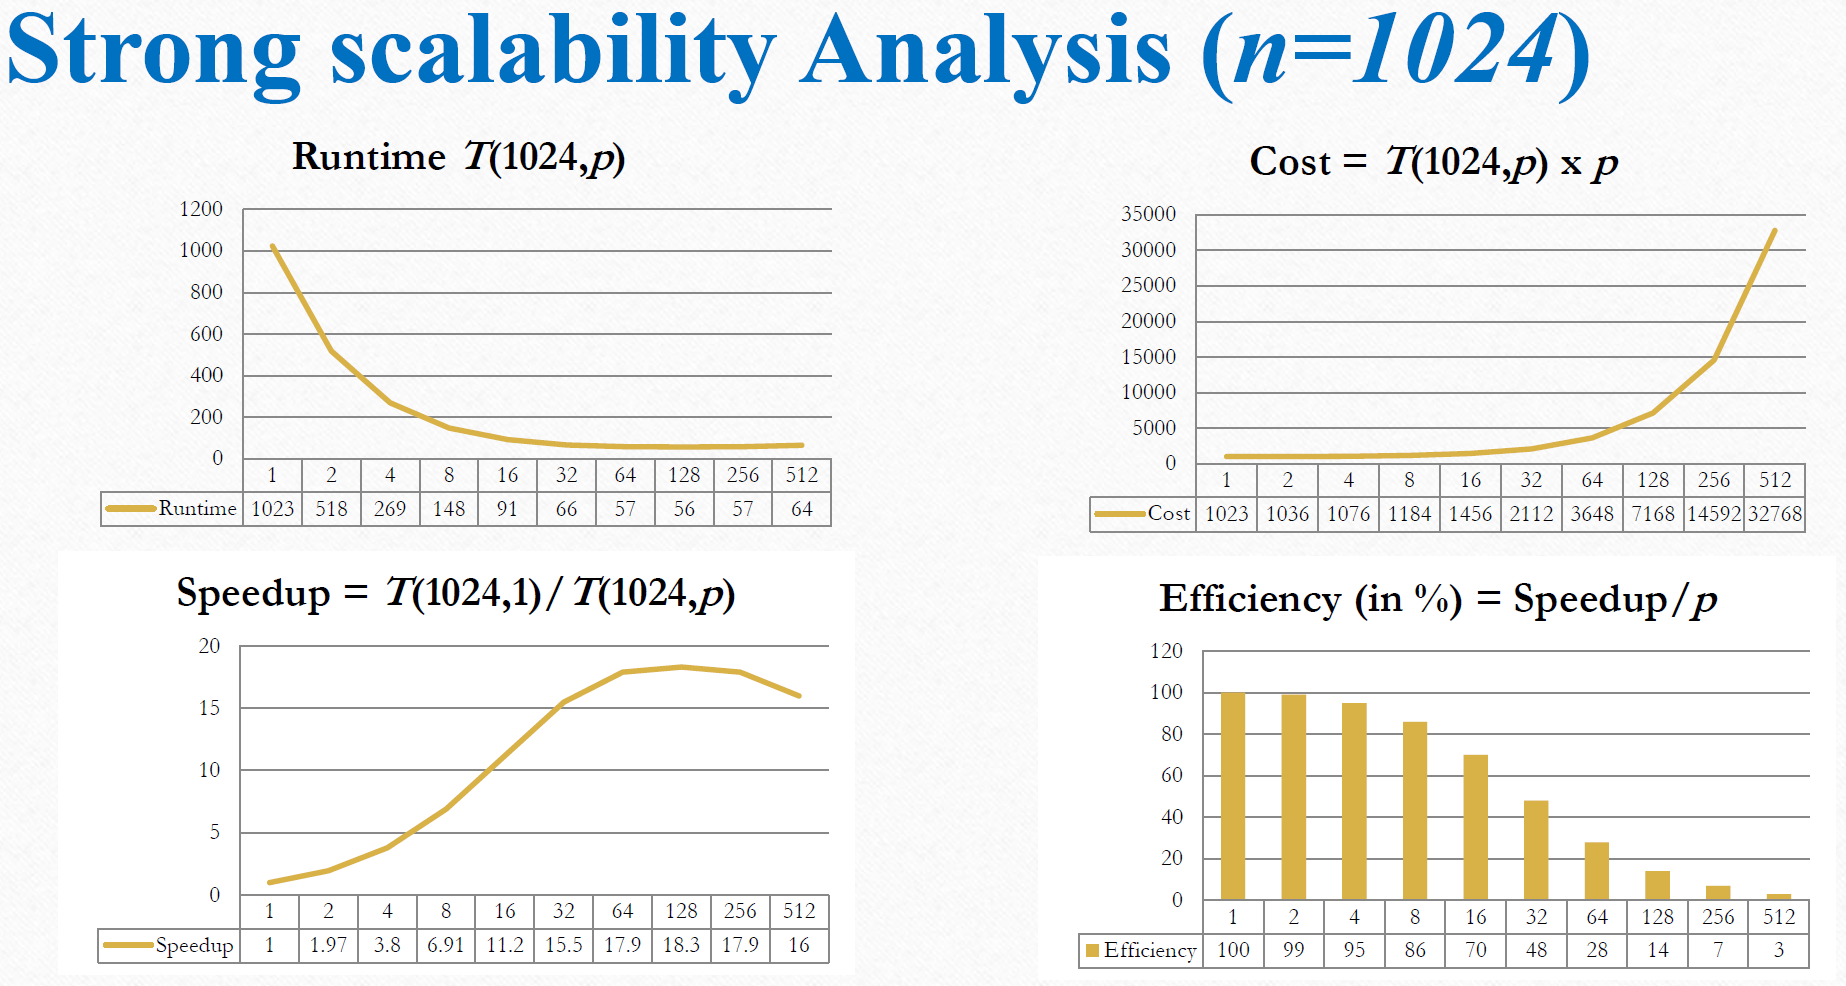
\includegraphics{images/06/scalability_analysis.png}
   \caption{Strong scalability analysis}
   \label{fig:06/scalability_analysis}
\end{figure}

We can determine which is the optimal speedup for a given problem. It is the red line in Fig. \ref{fig:06/optimal_speedup} .
\begin{figure}[htbp]
   \centering
   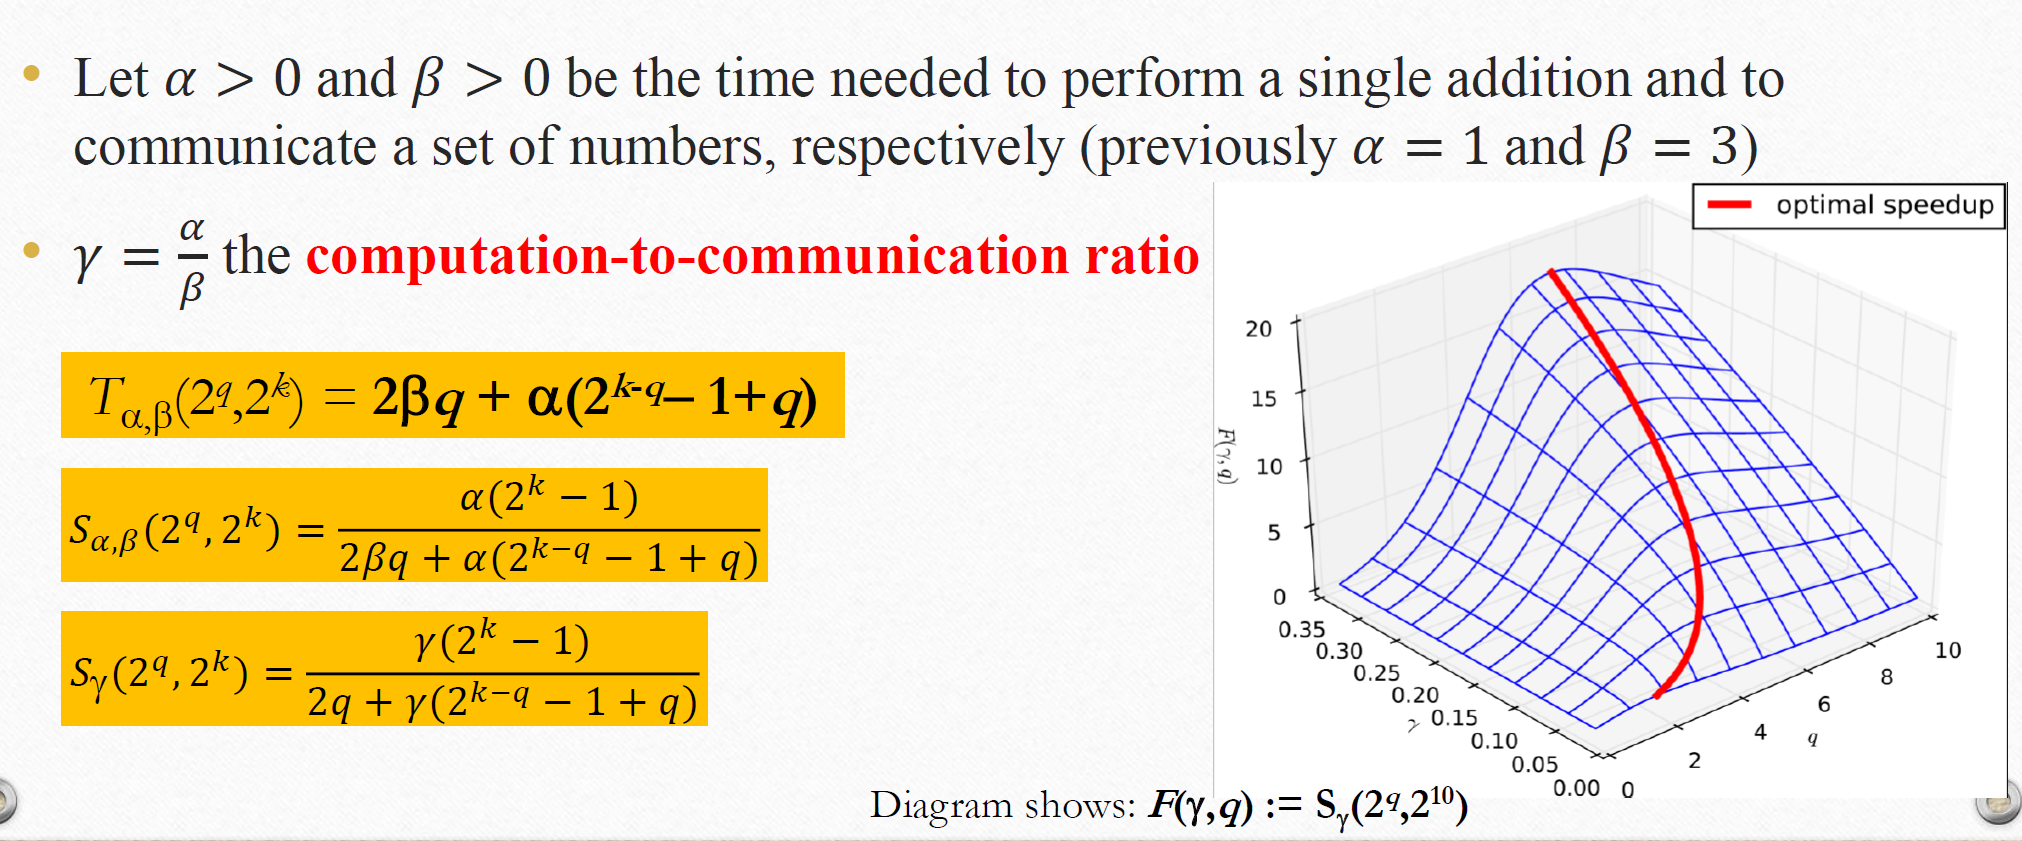
\includegraphics{images/06/optimal_speedup.png}
   \caption{Computation-to-communication ratio}
   \label{fig:06/optimal_speedup}
\end{figure}

\framedt{Takeaway message}{
   In general the speedup is mostly stable up to a certain point, then it starts to decrease. This is due to the fact that the communication overhead starts to dominate the computation time.

   The grater the communication overhead, the lower the speedup.
}


\section{Laws of Parallel Systems}

\subsection{Amdahl's Law}

It states that \ul{no matter how many processors are used in a parallel run, the program's speedup will be limited by its fraction of sequential code.}\\
The Amdahl’s law gives an \textbf{upper bound} on the speedup that can be achieved.
The speedup is limited by the part of the task that cannot be parallelized. Even if you have a large number of processors, the sequential portion of the task becomes the bottleneck.
For example, if 90\% of the task can be parallelized, the maximum speedup (no matter how many processors) is limited to 10x, because the remaining 10\% has to be done sequentially.

\begin{definition}
   [Amdahl's Law]
   \begin{equation}
      S(p) = \frac{1}{f + \frac{1-f}{p}}
   \end{equation}
   where $f$ is the fraction of the program that is sequential. Conversely, $1-f$ is the fraction of the program that can be parallelized.
\end{definition}

However, note that Amdahl's law is not always applicable. In fact, it is based on the assumption that the problem size is fixed (\textbf{strong scalability}), and that the parallel part of the program is perfectly parallelizable.

\subsection{Gustafson's Law}

Gustafson's law takes into account scenarios where the problem size scales with the number of processors (\textbf{weak scalability}).
Unlike Amdahl's Law, Gustafson's Law assumes that the problem size grows with the number of processors, meaning that parallel processors are used to solve bigger problems rather than trying to reduce the execution time of a fixed problem size.As the problem grows, the parallelizable portion becomes more significant, leading to better utilization of the available processors.\\
The law asserts that the parallelizable part grows linear in p while the non-parallelizable part remains constant.

\begin{equation}
   S(p) \leq f + p(1-f) = p + f\cdot(1-p)
\end{equation}